\documentclass[Orbiter Developer Manual.tex]{subfiles} 
\begin{document}

\section{Spacecraft design}
This section describes how to create a new \textit{vessel class} for Orbiter by writing a \textit{vessel DLL module}. Although it is possible to create simple vessel classes by writing a vessel configuration file without a custom module, the full potential of Orbiter’s custom spacecraft design capabilities can only be realised with a specialised module.\\

\alertbox{All vessels of a given class share the same DLL module. Orbiter only loads a single instance of the DLL. This means that global variables are shared between all vessels of that class. Do not store data which are specific to individual vessels in global or static variables, because they can be overwritten by another vessel.}


\subsection{Module initialisation}
When the user launches the simulation by picking a scenario from the Orbiter Launchpad dialog and pressing the “Launch Orbiter” button, Orbiter will load the vessel DLL module for each spacecraft type used in the simulation, and call its \textit{InitModule} function. This function is called only once per Orbiter session, no matter how many spacecraft of that type appear in the simulation. It will not be called again if the user exits the simulation to the Launchpad, and reloads another simulation scenario. You can use it to initialise global (non-instance specific and non-session specific) parameters.

\begin{lstlisting}
#define ORBITER_MODULE
#include "orbitersdk.h"

HINSTANCE g_hDLL;

DLLCLBK void InitModule( HINSTANCE hModule )
{
	g_hDLL = hModule;
	// perform global module initialisation here
}
\end{lstlisting}

\noindent
In this example, we use the \textit{InitModule} function to save the module instance handle passed to the function in global variable \textit{g\_hDLL}. This handle is useful later, e.g. when loading resources stored in the module file. Note the first line of the code example, which defines the \textit{ORBITER\_MODULE} flag. This flag should be included in all Orbiter DLL modules, to ensure proper execution of initialisation and cleanup functions.\\
\\
At the end of a simulation run, Orbiter calls the \textit{ExitModule} function for each DLL module.

\begin{lstlisting}
DLLCLBK void ExitModule( HINSTANCE hModule )
{
	// perform module cleanup here
}
\end{lstlisting}

\noindent
If you performed any dynamic memory allocation in \textit{InitModule}, this is a good place to perform the corresponding cleanup operations which de-allocate that memory.


\subsection{Vessel initialisation}
To allow initialisation of individual spacecraft, Orbiter will call the ovcInit function each time a scenario is loaded, for each vessel of that type listed in the scenario file. Orbiter will also call \textit{ovcInit} during the simulation if a new vessel of this type is created. The main purpose of ovcInit is to create an instance of a \textit{VESSEL}-derived interface class. \textit{VESSEL} is a class defined in the Orbiter API which is the primary means of communication between Orbiter and your own spacecraft class. In order to make use of the interface, you should derive your own vessel class derived from \textit{VESSEL}. In \textit{ovcInit}, you then create an instance of that class and return it back to Orbiter. Note that in the latest Orbiter version, the new \textit{VESSEL2} class has been introduced which inherits all the methods of \textit{VESSEL}, and introduces a number of new callback functions which replace the previous method of event notification. You should derive your vessel class from \textit{VESSEL2} to make use of this latest interface.\\
\\
As an example, let’s create a new class called \textit{MyVessel}, and create an instance in \textit{ovcInit}:

\begin{lstlisting}
class MyVessel: public VESSEL2
{
	public:
		MyVessel( OBJHANDLE hObj, int fmodel ) : VESSEL2( hObj, fmodel ) {}
		~MyVessel() {}
		// add more vessel methods here
};

DLLCLBK VESSEL* ovcInit( OBJHANDLE hvessel, int flightmodel )
{
	return new MyVessel( hvessel, flightmodel );
}
\end{lstlisting}

\noindent
\textit{ovcInit} passes two parameters to your module: a handle to the vessel for which you are about to create an interface, and a flag for the type of flight model requested by the user. Both parameters are passed on to the vessel constructor. The vessel handle is required to identify your vessel when requesting information from Orbiter. The \textit{flightmodel} flag can be used to implement different behaviour in your module, for example to define an “easy” and a “complex” flight model, which can then be selected by the user. You don’t need to store these parameters in your module, because you can retrieve them with the \textit{GetHandle} and \textit{GetFlightModel} methods of the \textit{VESSEL} class.\\
\\
To ensure proper cleanup at the end of a simulation session, you must implement the \textit{ovcExit} function to delete your vessel:

\begin{lstlisting}
DLLCLBK void ovcExit( VESSEL* vessel )
{
	if (vessel) delete (MyVessel*)vessel;
}
\end{lstlisting}

\noindent
Note that you need to cast the generic \textit{VESSEL} pointer passed by Orbiter to your own vessel class to ensure that the correct destructors are called.


\subsection{Reading and saving a vessel state}
% TODO

\subsection{Defining class capabilities}
% TODO

\subsection{Creating rocket engines}
To propel your ship in space, you must equip it with engines. There exist a variety of different rocket engine types, such as liquid and solid fuel engines, or more futuristic ones such as ion or photon drives.

\subsubsection{A bit of theory}
\textbf{Thrust force}\\
\\
Despite their very different design, all engines work by the same principle: generating a thrust force in one direction by expelling particles in the opposite direction at high velocity. A liquid-fuel engine, for example, consists of a burn chamber in which a mixture of propellant and oxydiser are ignited, and a nozzle through which the expanding gas is forced at high velocity. The force $F_{th}$ generated by the engine is proportional to the propellant mass flow dm/dt and the velocity $v_{0}$ of the expelled gas:

\[ \vec{F}_{th} = \frac{dm}{dt} (t) \vec{v}_{0}\]

\noindent
When creating a thruster, you need to specify the maximum force $F_{th}$ it can generate when it is driven at full power, and the propellant exit velocity $v_{0}$. (in Orbiter, $v_{0}$ is called the \textit{fuel-specific impulse}, or Isp). The Isp value determines how much fuel per second is consumed to obtain a given thrust force. The higher the Isp value, the more fuel-efficient the engine.\\

\begin{figure}[H]
  \centering
  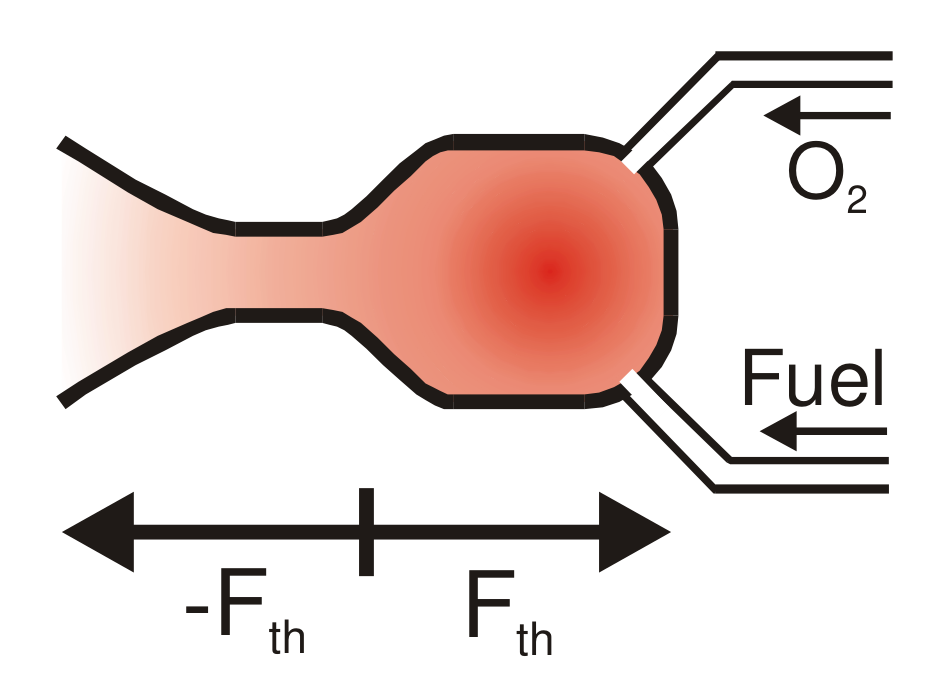
\includegraphics[width=0.5\hsize]{engine.png}
\end{figure}

\noindent
Sometimes the \textit{thrust-specific fuel consumption} (TSFC) is quoted in the literature. This is the amount of propellant that needs to be burned per second to obtain 1N of thrust. Thus the TSFC is the inverse of the Isp and has units of [$s \ m^{-1}$], or more intuitively [$kg \ s^{-1} N^{-1}$].\\
\\
\textbf{Note:} In Orbiter, the thrust is specified as a force, and has units of Newton [$1N = 1kg \ m \ s^{-2}$]. In the literature, thrust is often specified in units of kg. To convert such data into Orbiter units, multiply by $1g = 9.81 \ m \ s^{-2}$. Isp is specified as a velocity in Orbiter, with units of $m \ s^{-1}$. In the literature it is often given in units of seconds [s]. To convert to Orbiter units, again multiply by 1g.\\
\\
\textbf{How long will my fuel last?}\\
\\
The burn time $T_{b}$ at full thrust $F_{max}$ for fuel mass $m_{F}$ is given by

\[ T_{b} = \frac{m_{F} \ Isp}{F_{max}} \]

\noindent
\textbf{Pressure-dependent thrust efficiency}\\
\\
Most conventional rocket engines work less efficiently in the presence of ambient atmospheric pressure, because the ignited gas must be expelled through the nozzle against the outside pressure of the atmosphere. This leads to a reduction of the thrust force at ambient pressure \textit{p}:

\[ F(p) = F_{0} - p A \]

\noindent
where $F_{0}$ is the vacuum thrust rating and A has units of an area [$m^{2}$] and can be regarded as the \textit{effective nozzle cross section}. If we know the force $F_{1}$ generated at ambient pressure $p_{1}$, then

\[ F_{1} = F_{0} - p_{1}A \ \Rightarrow \ A = \frac{F_{0} - F_{1}}{p_{1}} \]

\noindent
and therefore

\[ F(p) = F_{0} - p\frac{F_{0} - F_{1}}{p_{1}} = F_{0}(1 - \frac{F_{0} - F_{1}}{F_{0}p_{1}}) = F_{0}(1 - p\eta) \]

\noindent
and likewise

\[ Isp(p) = Isp_{0}(1 - p\eta) \]

\noindent
In the literature, the pressure-dependency of engine thrust is often defined by specifying the Isp value for both vacuum and a given reference pressure (e.g. atmospheric pressure at sea level). Orbiter uses the same convention to apply pressure dependency.\\
\\
\textbf{Thrust level}\\
In Orbiter, thrusters can be driven at any level L between 0 (cutout) and 1 (full thrust). The actual thrust force generated by the engine is thus calculated as

\[ F(p) = F_{max}(p) \cdot L \]

\noindent
In reality, thrusters can often only be driven at maximum, or within a limited range below maximum. This is not currently implemented in Orbiter, but may be introduced in a future version.\\
\\
\textbf{Thruster placement and thrust direction}\\
\\
The effect of a thruster depends on its placement on the vessel, and the direction in which the thrust force is generated. In the most general case, a thruster will produce both a linear acceleration (due to a force) and an angular acceleration (do to torque).\\
Torque is generated if the force vector does not pass through the vessel’s centre of gravity (CG)

\begin{figure}[H]
  \centering
  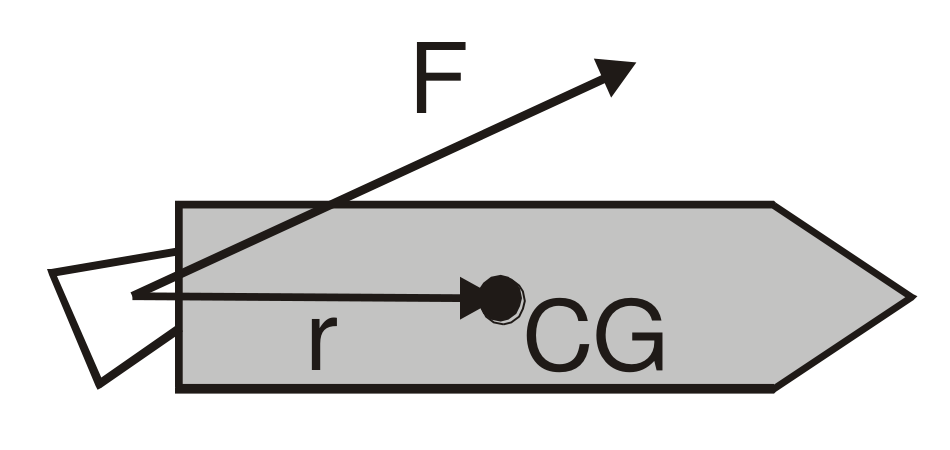
\includegraphics[width=0.5\hsize]{rocket_thrust.png}
\end{figure}

\noindent
The torque is then given by the cross product

\[ \vec{M} = \vec{F} \times \vec{r} \]

\noindent
(remember that Orbiter uses a left-handed coordinate system!) To avoid uncontrollable spin you should design your ship’s main engines so that their force vector passes through the CG. Vessel coordinates are always defined so that the CG is at the origin (0,0,0). Therefore, a thruster located at (0,0,-10) and generating thrust in direction (0,0,1) would not generate torque.\\
\\
\textbf{Attitude thrusters: Rotation}\\
\\
Sometimes generating torque is desired in order to rotate the spacecraft. For controlled attitude manouevres one then usually wants to change only the angular moment, without also inducing a linear acceleration. This requires the simultaneous operation of at least 2 thrusters so that their linear moments cancel.

\begin{figure}[H]
  \centering
  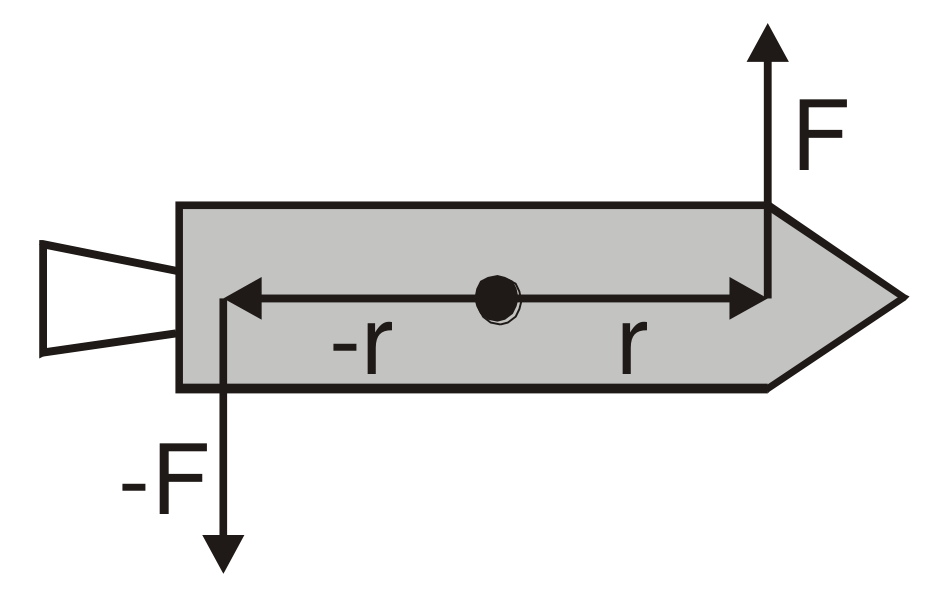
\includegraphics[width=0.5\hsize]{rocket_rotation.png}
\end{figure}

\noindent
\textbf{Attitude thrusters: Translation}\\
\\
In order to provide small linear accelerations in various directions (for example, to line the ship up with the docking port of a space station), thrusters must be driven single or in groups so that they don’t generate torque. Sometimes it is possible to re-use the rotational attitude thrusters for this task, but it is equally possible to add separate linear thrusters.\\

\begin{figure}[H]
  \centering
  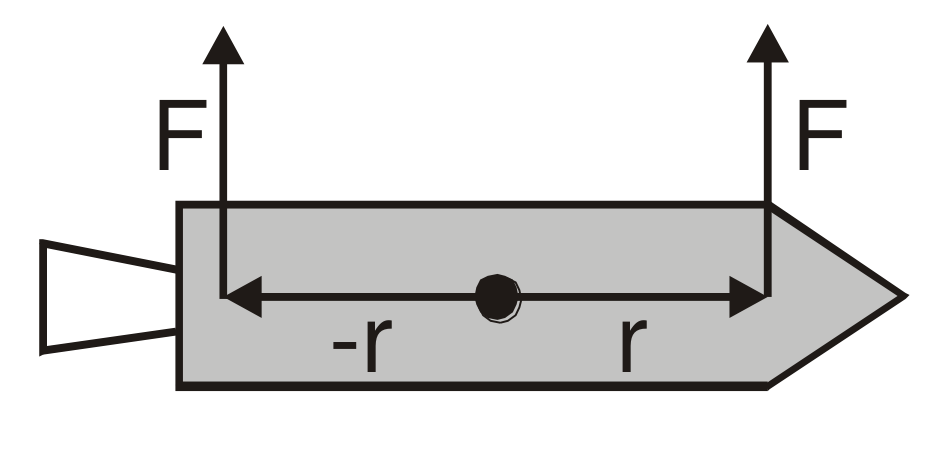
\includegraphics[width=0.5\hsize]{rocket_translation.png}
\end{figure}

\noindent
\textbf{Engine gimbal and thrust vectoring}\\
\\
Using attitude thrusters in a launch vehicle during the burn phase of the main engines is usually not practical. Instead, attitude control is performed by tilting the main engines and thereby generating a torque as described above. In practice this may be done by suspending the engines in a gimbal system which allows rotation around one or two axes. In Orbiter, this can be implemented by modifying the thrust direction of the engine.\\
\\
Another way to change the thrust direction is by inserting deflector plates into the exhaust stream.\\
\\
\textbf{Torque, angular momentum and angular velocity}\\
\\
The relationship between torque M and angular velocity is given by Euler’s equations for a rotating rigid body:
% TODO fix spacing between equations (2 and 3 show closer to each other than 1 and 2)
\[ J_{x}\dot{\omega}_{x} = M_{x} - (J_{z} - J_{y})\omega_{y}\omega_{z} \]
\[ J_{y}\dot{\omega}_{y} = M_{y} - (J_{x} - J_{z})\omega_{z}\omega_{x} \]
\[ J_{z}\dot{\omega}_{z} = M_{z} - (J_{y} - J_{x})\omega_{x}\omega_{y} \]

\noindent
where ($J_{x}$, $J_{y}$, $J_{z}$) are the principal moments of the inertia tensor (PMI), ($M_{x}$, $M_{y}$, $M_{z}$) are the components of the torque tensor, and ($\omega_{x}$, $\omega_{y}$, $\omega_{z}$) are the angular velocity components around the x, y, and z-axes. In Orbiter, this system of differential equations is solved by a trapezoid rule.


\subsubsection{Putting it all into the module}
% TODO

\subsubsection{Defining exhaust flames}
% TODO

\subsection{Air-breathing engines}
% TODO

\subsection{Rendering re-entry flames}
% TODO

\subsection{Adding particle streams for exhaust and reentry effects}
% TODO

\subsection{Atmospheric flight model}
% TODO

\subsection{Defining an animation sequence}
% TODO

\subsection{Designing 2D-instrument panels}
% TODO

\subsection{Designing instrument panels (legacy style)}
% TODO

\subsection{Designing virtual cockpits}
% TODO

\end{document}
